\documentclass[12pt]{article}
\usepackage{geometry}
\geometry{a4paper, lmargin=35mm,rmargin=30mm,tmargin=30mm,bmargin=30mm}
\usepackage{setspace}
\onehalfspacing
\usepackage{listings}
\usepackage{xcolor}
\usepackage{pgf-umlsd}
\usepackage{subcaption}
\usepackage{hyperref}
\usepackage{graphicx}
\graphicspath{ {./} }

\usepackage{tabularx}
\newcolumntype{b}{X}
\newcolumntype{s}{>{\hsize=.5\hsize}X}

\definecolor{codegreen}{rgb}{0,0.6,0}
\definecolor{codegray}{rgb}{0.5,0.5,0.5}
\definecolor{codepurple}{rgb}{0.58,0,0.82}
\definecolor{backcolour}{rgb}{0.95,0.95,0.92}
\lstdefinestyle{mystyle}{
    backgroundcolor=\color{backcolour},
    commentstyle=\color{codegreen},
    keywordstyle=\color{magenta},
    numberstyle=\tiny\color{codegray},
    stringstyle=\color{codepurple},
    basicstyle=\ttfamily\footnotesize,
    breakatwhitespace=false,
    breaklines=true,
    captionpos=b,
    keepspaces=true,
    numbers=left,
    numbersep=5pt,
    showspaces=false,
    showstringspaces=false,
    showtabs=false,
    tabsize=2
}
\lstset{style=mystyle}

\title{Emulation Framework for\protect\\ AIoT Federated Learning}
\author{Brendan Ang Wei Jie}
\begin{document}

\maketitle

\pagebreak
\section{Abstract}
Federated Learning (FL) allows a fleet of devices to collaborate towards a globally trained machine
learning model. Research has continued to produce novel algorithms to tackle
different issues faced in FL such as data heterogeneity and network costs. The performance
of these algorithms depend, in part, on the system parameters used
such as the number of clients participating in each round as well as real world factors such as
client drop off. However, measuring this performance through a realistic benchmark would require
one to procure a large fleet of devices which is infeasible and costly. Therefore, the role of
software simulation is to support researchers with the tools to do so. This work introduces a
software emulation framework utilizing QEMU and the Zephyr OS to
streamline the process of building a fleet of clients and allow validation testing of FL system
parameters that is not hardware-agnostic.
\pagebreak
  \section{Acknowledgements}
  I would like to thank Associate Prof Tan Rui, who provided me with this unique opportunity to work
  on such an interesting problem and for guiding me throughout the entire journey with new and
  refreshing ideas. Special thanks goes to my
  partner for her unwavering support and critical role as my proofreader.
\pagebreak
\tableofcontents
\listoffigures
\pagebreak

\section{Introduction}
Federated Learning (FL) emerged as a method for solving key issues with the standard centralized learning
approach, namely, it achieves the following properties:
\begin{itemize}
  \item Data Privacy: a centralized training approach involves the need for the centralized
    machine performing the computation to have full access to the entire data set. With FL, data never
    leaves each individual client's device. Instead, only the updated weights are shared to form the
    global model.
  \item Scalability: FL enables leveraging a network to perform computation in parallel.
\end{itemize}

These properties makes FL widely used in in the context of Artificial Intelligence of Things
(AIoT) devices. By leveraging the vast amount of data generated by IoT devices, FL harnesses the
collective intelligence of edge devices while respecting data sovereignty and privacy
regulations.\\

While FL has been successful in these aspects, there are a few limitations to the approach which may
not make FL practical in some applications. In particular, the distributed nature of FL poses a few key challenges:

\begin{itemize}
  \item Limited computing resources: individual devices may face memory constraints, limiting the
    size of the local model it is able to train. Constraints on computing power also lead to
    longer training times. This is particularly so for low-powered IoT devices.
  \item Network limitations: communication speed can become the bottleneck for performance as IoT
    devices rely on unstable wireless communication networks. Furthermore, data constraints can
    exist such that the number of bytes sent may be a cost inducing factor.
\end{itemize}

Hence, the development of FL algorithms often seek to advance progress towards solving the
aforementioned issues.

\subsection{Problem}
Prior to effectively deploying FL, different factors including the convergence rate and
model accuracy needs to be well studied. This gives rise to the need for software simulation. However, the
simulation of FL in the distributed setting involves dealing with
issues which do not arise in datacenter ML research. These include running on different simulated
devices, each with potentially varying amounts of data. Furthermore, metrics such as the number of
bytes transferred by the device, as well as the ability to simulate real-world issues such as client
drop-out, can also be important for proposed FL algorithms to handle.

difference between pre-trained and on-device training

\subsection{Literary Review}
FLSim\cite{li_2021_flsim} aims to provide a simulation framework for FL by offering its users a set
of software components --
which can then be mixed and matched to create a simulator for their use case. Developers need only
define the data, model and metrics reported, and FL system parameters can be altered in a JSON
configuration file. FLUTE\cite{garcia_2022_flute} adds additional features by allowing users to gain access to cloud based
compute and data. However, these simulation solutions are consequently hardware-agnostic. Without
taking into account the specific platforms which FL is performed on, these simulators cannot provide
insight into whether the system will work in the production environment.\\

In contrast, FedML\cite{he_2020_fedml} is a research-oriented library which supports various algorithms and 3 platforms, on-device training for IoT and
mobile devices, distributed computing and single-machine simulation.
Simulation is offered through the FedML Parrot\cite{tang_2023_fedml}, which offers an accelerated simulation
framework employing multiple optimizations to improve simulation speed.
However, on-device training is supported only on Raspberry Pi 4 and NVIDIA Jetson Nano which limits
hardware validation to these 2 devices.\\

One approach to acquiring hardware dependent results is to emulate the hardware environment. This
can be achieved through software systems. One such system explored the combination of Quick Emulator (QEMU)
and Zephyr, a real time operating system to emulate embedded devices in the FL contenxt\cite{ntu}. However,
this approach only emulated machine learning inference rather than on-device training.\\

Here, this work proposes a new emulation framework ``zfl'', which aims to achieve the following
properties:
%TODO: LINK BACK TO THESE AIMS
\begin{itemize}
  \item Provide better insight into hardware specific support by running FL on emulated hardware
    through QEMU and Zephyr OS.
  \item Collect useful metrics during the FL lifecycle.
  \item Support simulation of real word issues such as variable data and client drop-off.
\end{itemize}

\subsection{QEMU}
QEMU\cite{qemu} is an open source machine emulator and virtualizer. It enables system emulation,
creating a virtual model of an entire machine (CPU, memory and emulated devices) to run a guest OS.
In this mode, the CPU may be fully emulated, or it may work with a hypervisor to allow the guest to
run directly on the host CPU. In zfl, QEMU with full CPU emulation is used without a hypervisor as
part of its software architecture to emulate hardware. Note that by default, the framework
is built for QEMU x86 32-bit, which entails the use of the qemu-i386 binary in section \ref{implementation}.

\subsection{Zephyr OS}
To emulate the issue of limited computing resources, it is important to make use of system runtimes
used by those devices. Zephyr OS\cite{zephyr} is one such operating system. It is based on a small-footprint kernel designed for use on resource-constrained
and embedded systems: from simple embedded environmental sensors and LED wearables to sophisticated embedded controllers, smart watches, and IoT wireless applications.
Furthermore, Zephyr is highly configurable, allowing the user to choose only the specific kernel
services required, and also delve into lower level memory mapping of the system SRAM and DRAM. Most
importantly, Zephyr supports a wide range of CPU architectures including ARM, RISC-V and x86.
Zephyr also provides built-in capabilities for building for the QEMU environment, and implements key
features such as networking through the QEMU built-in Ethernet adapter. In zfl,
client code will be written to work in the Zephyr OS environment.

\section{Implementation}\label{implementation}
The framework implements the classical FedAvg algorithm\cite{brendan_2016_communicationefficient} as part of
its simulation, where each client sends its updated model weights to a central server, which then performs aggregation
using simple averaging. Hence, the architecture of the framework is based on the assumption of
multiple clients talking to a single server.\\

To run on Zephyr OS, the entire software stack is developed in the C programming language. Although
Zephyr also supports applications written in C++, the C programming language would make the framework
more suitable to run on embedded devices. Note that the framework is implemented for Linux and all tests are run
on a Debian based machine.

\subsection{Configuration}
In order to run machine learning training on each client, some configuration is required to ensure
that we have sufficient memory to allocate for the neural network model and training data. Depending
on the architecture of the model and the size of the data, these options may need to be further tweaked to
prevent any runtime memory allocation crashes. Listing \ref{lst:prj.conf} shows the options made to
\verb|prj.conf| to create a runtime capable of up to 10MB of heap memory. Listing
\ref{lst:board} shows
the configuration made to the QEMU board under \verb|qemu_x86.dts| for a total DRAM size of 15MB.
This is in excess of the heap memory size as additional memory is reserved for the kernel image and
stack memory.\\

\begin{minipage}[b][][b]{.45\textwidth}
\begin{lstlisting}[language=bash,caption={Zephyr prj.conf},label={lst:prj.conf}]
CONFIG_SRAM_SIZE=15360
CONFIG_MAIN_STACK_SIZE=8192
CONFIG_KERNEL_VM_SIZE=0x7000000
CONFIG_HEAP_MEM_POOL_SIZE=10485760
\end{lstlisting}
\end{minipage}\hfill
\begin{minipage}[b][][b]{.45\textwidth}
\begin{lstlisting}[language=C,caption={QEMU board.dts},label={lst:board}]
#define DT_DRAM_SIZE DT_SIZE_K(15360)
\end{lstlisting}
\end{minipage}

The main zfl binary is used to bootstrap either the client or server aspects of FL simulation.
Listing \ref{lst:bootstrap} shows the different options available for configuring FL parameters and
their meanings.
\begin{lstlisting}[language=bash,caption={The main zfl binary},label={lst:bootstrap}]
./zfl client -c num_clients -e epochs -b batch_size
# -c num_clients: Number of clients to boot up.
# -e epochs:      Number of epochs (training passes on the entire data set).
# -b batch_size:  Number of training labels used for a single update.

./zfl server -r num_rounds -c clients_per_round
# -r num_rounds:        Number of rounds of aggregation.
# -c clients_per_round: Number of clients that need to respond to start a round.
\end{lstlisting}

\subsection{Bootstrapping Process}
Next the framework needed a method for spawning an arbitrary number of QEMU instances, and allowing
these instances to communicate back to the server. When called in client mode (Listing
\ref{lst:fork}), zfl accomplishes this
by making use of the ``fork'' and ``exec'' pattern with the desired number of clients. \\

However, each instance of QEMU persists in an isolated network different from the host PC,
and is not able to communicate. We can bypass this limitation using a network bridge to act as a
virtual network device forwarding packets between connected network devices.
The network bridge is set up on the host under the name ``zfl'' with a set of network parameters using
the \verb|ip| command line utility as shown in Listing \ref{lst:ip}.
\begin{lstlisting}[language=bash,caption=Network bridge setup,label={lst:ip}]
ip link add $INTERFACE type bridge
ip addr add $IPV4_ADDR_1 dev $INTERFACE
ip link set enp61s0 master $INTERFACE
ip route add $IPV4_ROUTE_1 dev $INTERFACE > /dev/null 2>&1
ip link set dev $INTERFACE up
\end{lstlisting}
To tell QEMU to use it, we pass the name of the bridge along
with a randomly generated MAC address as arguments to the \verb|-nic| flag:
\begin{verbatim}
  -nic bridge,model=e1000,mac=%s,br=zfl
\end{verbatim}

Although each QEMU client is now able to communicate with the host via the NIC adapter, we still
needed a way to monitor the output of each instance. One method is to transmit
output and logs over the network. However, this would not allow important crash logs and stacktrace
information to be transmitted as the application software would have shutdown. To overcome this, the host
creates a named or FIFO pipe for each client, which then is passed into
QEMU through the \verb|-serial| flag. Now, all standard output goes through the named pipe, ready to be read
by the host. Another outcome of this is that the host is also able to send input to each
instance, whose importance will be described in the next section. Listing \ref{lst:fork} showcases
how each feature is configured through the QEMU command line binary.

\begin{lstlisting}[language=C,caption=Client forking process,label={lst:fork}]
pid_t child = fork();
if (child < 0) {
    printf("ERROR: could not fork client %d: %s\n", i, strerror(errno));
    return 1;
}
...

// generate serial arguments
char serial_arg[80];
snprintf(serial_arg, 80, "pipe:%s", pipe_path);

// generate nic arguments
char nic_arg[100];
char *mac = generate_random_mac();
snprintf(nic_arg, sizeof(nic_arg), "bridge,model=e1000,mac=%s,br=zfl", mac);

// start client as new process
execlp("qemu-system-i386", "qemu-system-i386",

       "-m", "15", "-cpu", "qemu32,+nx,+pae", "-machine", "q35",
       "-device", "isa-debug-exit,iobase=0xf4,iosize=0x04",

       "-no-reboot", "-nographic", "-no-acpi",

       "-serial", serial_arg,

       "-nic", nic_arg,

       "-kernel", "./zflclient/out/zephyr/zephyr.elf",

       NULL);
\end{lstlisting}

In addition to the NIC adapter configuration, each client needed a unique Internet Protocol Version
4 (IPv4) address in order to establish TCP based connections with the central server. Samples
provided by Zephyr OS describe a way to achieve this by setting a compile time configuration flag\\
\verb|CONFIG_NET_CONFIG_MY_IPV4_ADDR|. However, this is impractical to scale to a large number of clients, since
each client would need a separately compiled binary. One solution to this problem is to assign the IPv4 address
dynamically using the built-in Zephyr network function\cite{schirrmeister_2020_simulation}:
\begin{verbatim}
net_if_ipv4_addr_add
\end{verbatim}
To achieve this, each client starts off as a Zephyr shell instance and a user-defined command
\verb|run| is registered. This exposes a shell command that takes in a command line argument which defines the desired IP address of the
instance (Listing \ref{lst:shellcmd}). Finally, this command triggers the run function
(Listing \ref{lst:run}) as a way to start the main program. \\

Overall, the complete emulation architecture is illustrated in figure \ref{fig:architecture},
describing the interactions between the host system and guest instances. \\

\begin{lstlisting}[language=C, caption=Registering user defined command ``run'' to the function
pointer run,label={lst:shellcmd}]
SHELL_CMD_ARG_REGISTER(run, NULL, "Run with IPv4 address", run, 4, 0);
\end{lstlisting}

\begin{lstlisting}[language=C, caption=The ``run'' function which performs IP address assignment at
runtime,label={lst:run}]
int run(const struct shell *sh, size_t argc, char **argv) {
    // ...
    char *addr_str = argv[1];
    LOG_INF("instance ipaddr is %s", addr_str);
    struct in_addr addr;
    zsock_inet_pton(AF_INET, addr_str, &addr);
    if (!net_if_ipv4_addr_add(net_if_get_default(), &addr, NET_ADDR_MANUAL, UINT32_MAX)) {
        LOG_ERR("failed to add %s to interface", addr_str);
        return -1;
    }
    // ...
}
\end{lstlisting}

\begin{figure}
  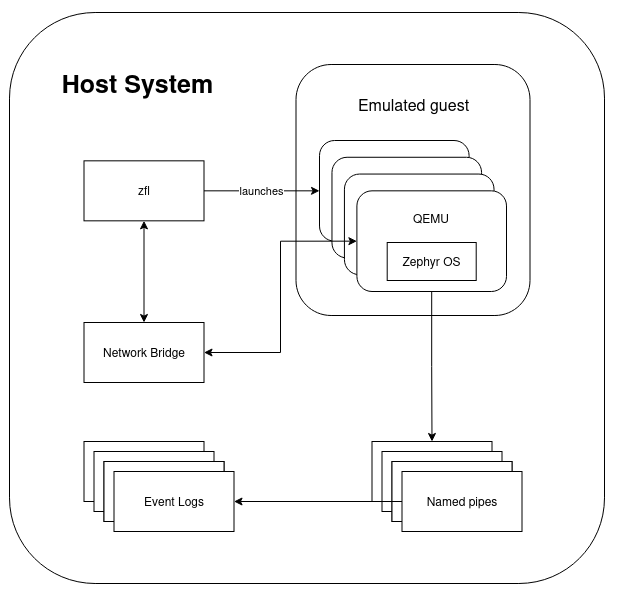
\includegraphics[scale=0.8]{architecture}
  \caption{Host-guest emulation architecture}
  \label{fig:architecture}
\centering
\end{figure}

\subsection{Client}
The first step within the internal implementation of each client is to establish TCP socket connection to the central server and obtain
their assigned ID. This is then used to obtain the training data from the server which corresponds
to that ID. Thus, this process allows for training data to be dynamically assigned to different
instances. Finally, each client starts a HTTP server and marks itself as ready to begin the training round.
The complete initialization process is illustrated in Figure \ref{fig:clientinit}.

\subsubsection{Machine Learning}
Once initialized, clients wait for a request to their \verb|start| HTTP endpoint. This triggers the
train function, which performs forwarding and backpropagation on the local data set.
The underlying neural network implementation utilizes nn.h\cite{_2024_tsodingnnh},
an open source educational neural network C library. Porting the library for use included updating
traditional POSIX syscalls to the Zephyr kernel syscalls. However, further modifications were made for specific use as described in
section \ref{experiments}. %TODO: talk more about the implications of these results

\begin{figure}
  \centering
  \begin{sequencediagram}
    \newinst{A}{Client}{}
    \newinst[2]{B}{Server}{}
    \begin{call}{A}{/id}{B}{id}
    \end{call}
    \begin{call}{A}{/training-data-i}{B}{data}
    \end{call}
    \begin{call}{A}{self.ready = true}{A}{}
    \end{call}
  \end{sequencediagram}
  \caption{Client initialization sequence}
  \label{fig:clientinit}
\end{figure}

\subsection{Server}
The central server runs on the host machine without needing additional configuration. Its primary
purpose is to aggregate individual client weights every round. Implemented HTTP endpoints are described in figure
\ref{fig:httpendpoints}. After assigning each connecting client their ID and training data, it performs the function
\verb|start_round| at an interval of 10 seconds. Each time, the server pings all previously
connected clients to check if they are ready to start the training round. When enough clients are
ready, it sends a HTTP POST request to the \verb|start| endpoint of the client, which then triggers the training
function. Once the client has completed its training, it sends the resulting weights of the local model
to the HTTP POST endpoint \verb|results| of the server, which then performs the aggregation. The
sequence of events for a single round is illustrated in Figure \ref{fig:flround}.

\subsubsection{Metrics}
As part of the framework's aim to track useful metrics, the server keeps track of the total number
of bytes transferred between the clients and itself during the entire FL lifecycle. The total
training time in seconds is also tallied. This is displayed along with additional details such as
the current round, number of ready clients, as well as a graph of the validation set loss and
accuracy on a simple graphical user interface shown in Figure \ref{fig:gui}.

\begin{figure}
  \centering
  \begin{sequencediagram}
    \newinst[1]{A}{Client i}{}
    \newinst[2]{B}{Server}{}
    \begin{call}{B}{/ready}{A}{true}
    \end{call}
    \begin{messcall}{B}{/start}{A}{}
    \end{messcall}
    \begin{messcall}{A}{/results}{B}{}
    \end{messcall}
  \end{sequencediagram}
  \caption{FL round}
  \label{fig:flround}
\end{figure}

\begin{figure}
\begin{tabularx}{\textwidth} {
  | >{\raggedright\arraybackslash}s
  | >{\centering\arraybackslash}s
  | >{\raggedright\arraybackslash}b | }
 \hline
 \multicolumn{3}{|c|}{Client} \\
 \hline
 Endpoint & HTTP Method & Description \\
 \hline
 /start & POST & Initiates training round using updated weights with JSON body: \newline\{weights: int\}  \\
 \hline
 /ready & GET & Gets client ready status \\
 \hline
 \multicolumn{3}{|c|}{Server} \\
 \hline
 /results?id= & POST & Client id submits results with JSON body: \newline\{round: int, weights: string\}  \\
 \hline
 /id & GET & Obtain an id for round participation \\
 \hline
 /training-data?id= & GET & Obtain training data for id \\
 \hline
 /training-labels?id= & GET & Obtain training labels for id \\
 \hline
\end{tabularx}
\caption{HTTP endpoints}
\label{fig:httpendpoints}
\end{figure}

\begin{figure}
  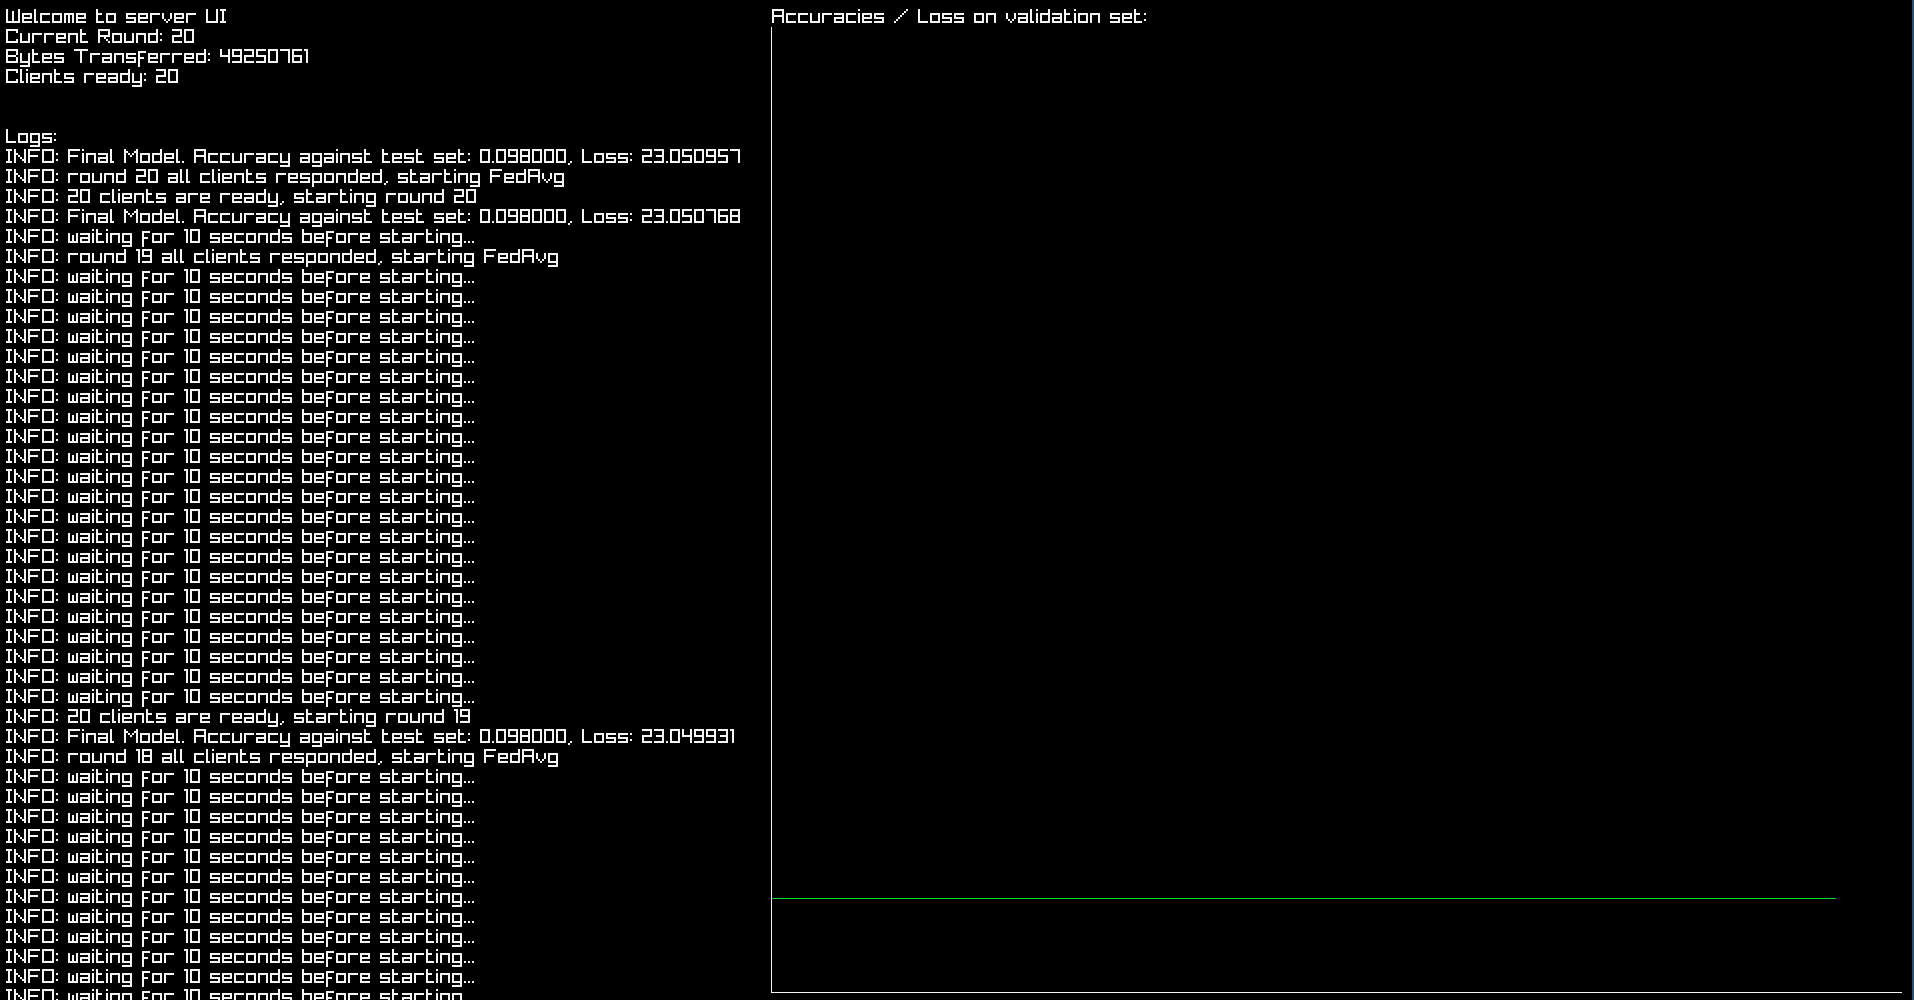
\includegraphics[scale=0.3]{gui}
  \caption{GUI Implementation}
  \label{fig:gui}
\centering
\end{figure}

\section{Experiments}\label{experiments}
The framework is tested using FedAvg over the MNIST digit recognition data set of 60000 labels. Due to memory
constraints, clients are configured with a neural network architecture with 1 hidden layer of 16
nodes. Additionally, implementations for the softmax activiation and cross entropy were made to
ensure suitability for machine learning with MNIST categorical data.\\

To test the sanity of the framework, the data is first shuffled and split equally into 100 sets of 6000 labels.
The server is started for 20 rounds and 100 clients per round and clients were started with 5 epochs and a batch size of 600.
Figure \ref{fig:loss} shows the validation set loss and Figure \ref{fig:accuracy} shows the
validation set accuracy at the end of each round. There can be many reasons for the lack of
accuracy gain. For one, the model architecture is very shallow, reducing each clients ability to
make significant steps towards their local minima. Furthermore, traditional FedAvg also suffers from
model inaccuracy caused by the loss of knowledge during model training\cite{hinton2015distilling}. Nevertheless, although the framework is unable to converge
towards an acceptable target accuracy during the experiment, a steadily decreasing cross entropy
loss helps to validate that the entire system is performing.

\begin{figure}
\begin{subfigure}{.5\textwidth}
  \centering
  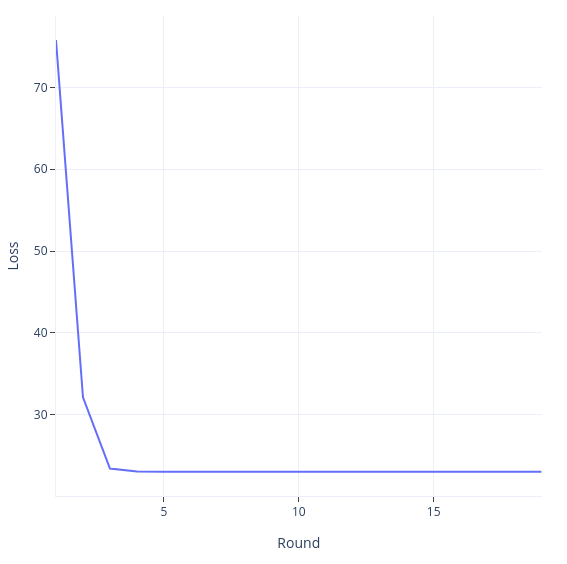
\includegraphics[scale=0.5]{loss}
  \caption{20 round validation set loss}
  \label{fig:loss}
\end{subfigure}
\begin{subfigure}{.5\textwidth}
  \centering
  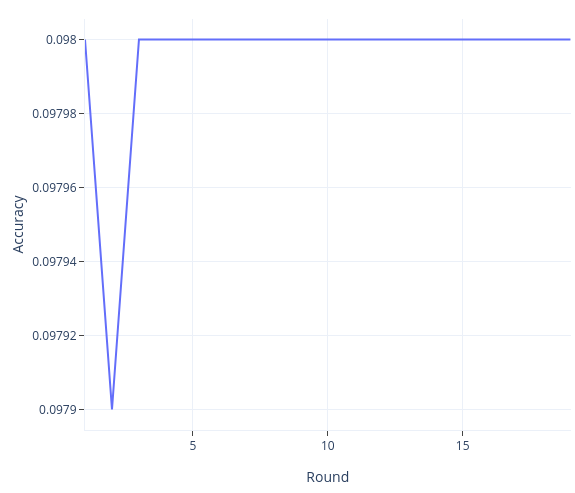
\includegraphics[scale=0.5]{accuracy}
  \caption{20 round validation set accuracy}
  \label{fig:accuracy}
\end{subfigure}
\end{figure}

\section{Limitations}
\subsection{Long training times}
Unoptimized client training implementations has resulted in long training times required per FL
round. This is because standard implementations for machine learning
algorithms that can be easily ported and suitable for use in Zephyr OS could not be found.
Traditional runtimes such as Tensorflow\cite{tensorflow2015-whitepaper} rely on the availability of a Python interpreter on
the device. Furthermore, these runtimes are usually not developed or optimized for resource
constrained environments, incurring a large binary size and high memory usage. However, there is
progress towards integrating Tensorflow Lite Micro into Zephyr OS through external modules
and has examples for running pre-trained neural network on their platform. However, on-device
training is still not supported.

\subsection{Limited algorithm support}
The framework currently only implements training algorithms for FedAvg. The architecture of zfl also
inherently assumes the use of a single server instance used for aggregation. However, this
limitation can be bypassed by porting specific HTTP endpoints from the server to the client. For
example, the implementation of the \verb|results| endpoint, would effectively move aggregation into
each client instance. This could potentially allow the framework to support hierarchical FL
algorithms\cite{rana_2023_hierarchical}.\\

Furthermore, future work could also look into implementing other FL algorithms in a bid to improve
the usability of the framework. These algorithms should aim to achieve higher model accuracy without
compromising on the requirements needed to function in an embedded low-powered device environment.
One example could be Distillation Based Federated Learning\cite{liu2022efficient}.

%TODO: CONCLUSION

\pagebreak
\bibliographystyle{IEEEtran}
\bibliography{refs}

\end{document}
